\documentclass{standalone}
\usepackage{tikz}
\usetikzlibrary{patterns, positioning}


\begin{document}
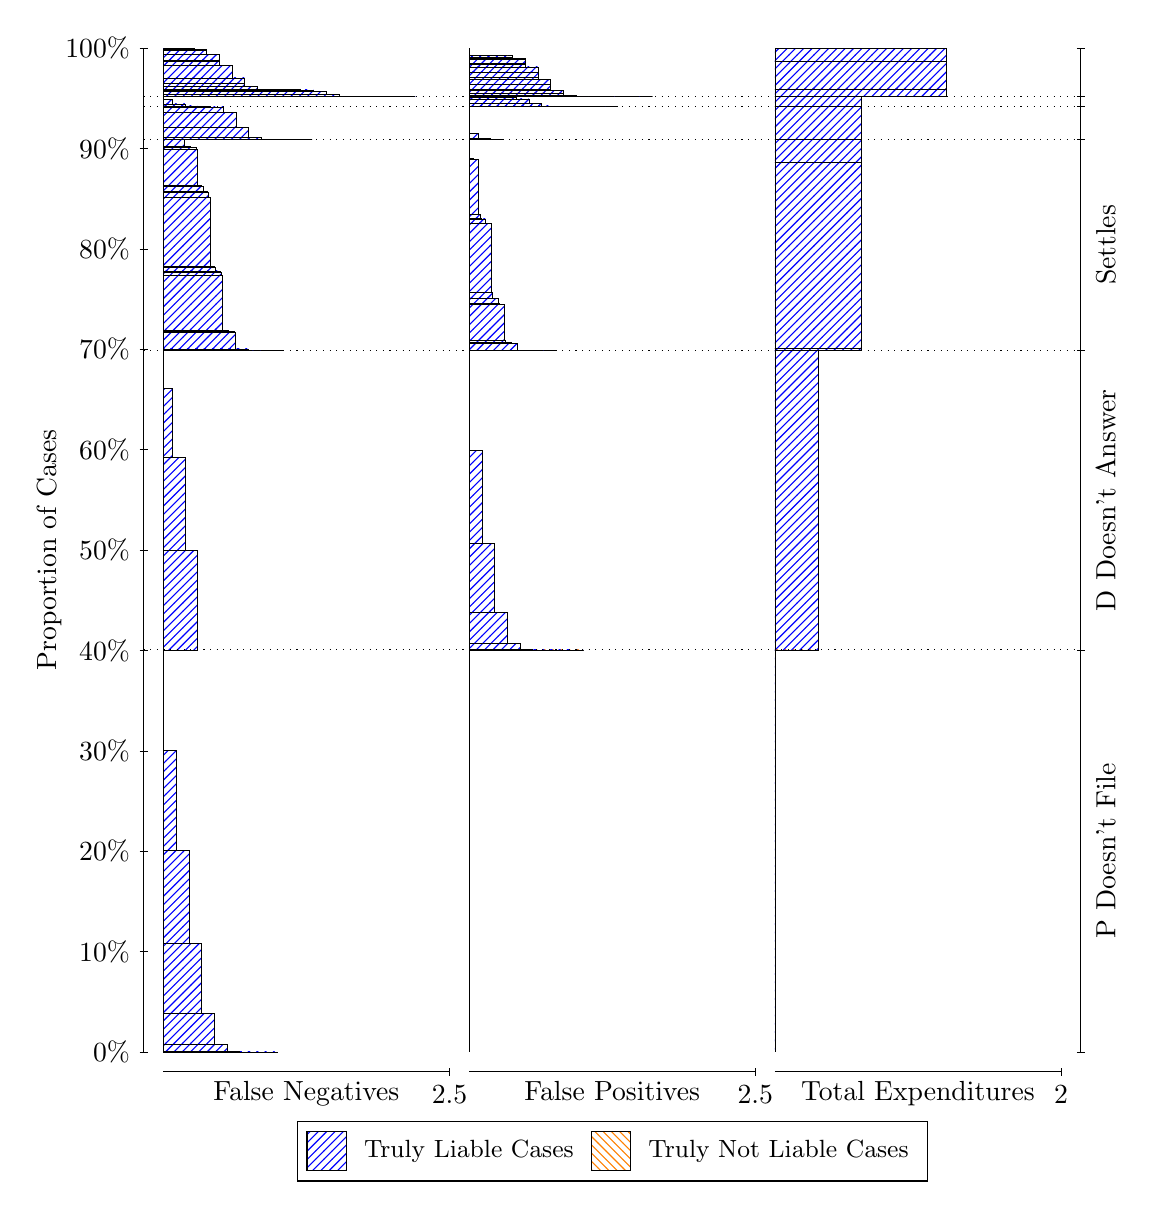
\begin{tikzpicture}
\draw[black, very thin] (1.5,1.75) -- (1.5,14.5);
\node[rotate=90, text=black, anchor=center] at (0.3, 8.125) {Proportion of Cases};
\draw[black, very thin] (1.45,1.75) -- (1.55,1.75);
\node[text=black, anchor=east] at (1.45, 1.75) {0\%};
\draw[black, very thin] (1.45,3.025) -- (1.55,3.025);
\node[text=black, anchor=east] at (1.45, 3.025) {10\%};
\draw[black, very thin] (1.45,4.3) -- (1.55,4.3);
\node[text=black, anchor=east] at (1.45, 4.3) {20\%};
\draw[black, very thin] (1.45,5.575) -- (1.55,5.575);
\node[text=black, anchor=east] at (1.45, 5.575) {30\%};
\draw[black, very thin] (1.45,6.85) -- (1.55,6.85);
\node[text=black, anchor=east] at (1.45, 6.85) {40\%};
\draw[black, very thin] (1.45,8.125) -- (1.55,8.125);
\node[text=black, anchor=east] at (1.45, 8.125) {50\%};
\draw[black, very thin] (1.45,9.4) -- (1.55,9.4);
\node[text=black, anchor=east] at (1.45, 9.4) {60\%};
\draw[black, very thin] (1.45,10.675) -- (1.55,10.675);
\node[text=black, anchor=east] at (1.45, 10.675) {70\%};
\draw[black, very thin] (1.45,11.95) -- (1.55,11.95);
\node[text=black, anchor=east] at (1.45, 11.95) {80\%};
\draw[black, very thin] (1.45,13.225) -- (1.55,13.225);
\node[text=black, anchor=east] at (1.45, 13.225) {90\%};
\draw[black, very thin] (1.45,14.5) -- (1.55,14.5);
\node[text=black, anchor=east] at (1.45, 14.5) {100\%};

\draw[black, very thin] (13.4,1.75) -- (13.4,14.5);
\draw[black, very thin] (13.35,1.75) -- (13.45,1.75);
\node[anchor=west] at (13.35, 1.75) {};
\draw[black, very thin] (13.35,6.8558) -- (13.45,6.8558);
\node[anchor=west] at (13.35, 6.8558) {};
\draw[black, very thin] (13.35,10.658) -- (13.45,10.658);
\node[anchor=west] at (13.35, 10.658) {};
\draw[black, very thin] (13.35,13.342) -- (13.45,13.342);
\node[anchor=west] at (13.35, 13.342) {};
\draw[black, very thin] (13.35,13.761) -- (13.45,13.761);
\node[anchor=west] at (13.35, 13.761) {};
\draw[black, very thin] (13.35,13.881) -- (13.45,13.881);
\node[anchor=west] at (13.35, 13.881) {};
\draw[black, very thin] (13.35,14.5) -- (13.45,14.5);
\node[anchor=west] at (13.35, 14.5) {};

\draw[black, very thin, pattern color=blue, pattern=north east lines] (1.75,1.75) rectangle (3.2033,1.75);
\draw[black, very thin, pattern color=blue, pattern=north east lines] (1.75,1.75) rectangle (3.0419,1.75);
\draw[black, very thin, pattern color=blue, pattern=north east lines] (1.75,1.75) rectangle (2.8804,1.7503);
\draw[black, very thin, pattern color=blue, pattern=north east lines] (1.75,1.7503) rectangle (2.7189,1.7587);
\draw[black, very thin, pattern color=blue, pattern=north east lines] (1.75,1.7587) rectangle (2.5574,1.8456);
\draw[black, very thin, pattern color=blue, pattern=north east lines] (1.75,1.8456) rectangle (2.3959,2.2417);
\draw[black, very thin, pattern color=blue, pattern=north east lines] (1.75,2.2417) rectangle (2.2344,3.1249);
\draw[black, very thin, pattern color=blue, pattern=north east lines] (1.75,3.1249) rectangle (2.073,4.3146);
\draw[black, very thin, pattern color=blue, pattern=north east lines] (1.75,4.3146) rectangle (1.9115,5.5812);
\draw[black, very thin, pattern color=orange, pattern=north west lines] (1.75,5.5812) rectangle (1.75,5.5812);
\draw[black, very thin, pattern color=blue, pattern=north east lines] (1.75,5.5812) rectangle (1.75,6.8558);
\draw[black, very thin, pattern color=blue, pattern=north east lines] (1.75,6.8558) rectangle (2.186,8.1193);
\draw[black, very thin, pattern color=blue, pattern=north east lines] (1.75,8.1193) rectangle (2.0245,9.3031);
\draw[black, very thin, pattern color=blue, pattern=north east lines] (1.75,9.3031) rectangle (1.863,10.182);
\draw[black, very thin, pattern color=orange, pattern=north west lines] (1.75,10.182) rectangle (1.75,10.182);
\draw[black, very thin, pattern color=blue, pattern=north east lines] (1.75,10.182) rectangle (1.75,10.658);
\draw[black, very thin, pattern color=blue, pattern=north east lines] (1.75,10.658) rectangle (3.276,10.658);
\draw[black, very thin, pattern color=blue, pattern=north east lines] (1.75,10.658) rectangle (3.2033,10.658);
\draw[black, very thin, pattern color=blue, pattern=north east lines] (1.75,10.658) rectangle (3.1307,10.658);
\draw[black, very thin, pattern color=blue, pattern=north east lines] (1.75,10.658) rectangle (3.1145,10.658);
\draw[black, very thin, pattern color=blue, pattern=north east lines] (1.75,10.658) rectangle (3.058,10.658);
\draw[black, very thin, pattern color=blue, pattern=north east lines] (1.75,10.658) rectangle (3.0419,10.658);
\draw[black, very thin, pattern color=blue, pattern=north east lines] (1.75,10.658) rectangle (2.9853,10.658);
\draw[black, very thin, pattern color=blue, pattern=north east lines] (1.75,10.658) rectangle (2.9692,10.658);
\draw[black, very thin, pattern color=blue, pattern=north east lines] (1.75,10.658) rectangle (2.953,10.658);
\draw[black, very thin, pattern color=blue, pattern=north east lines] (1.75,10.658) rectangle (2.8965,10.658);
\draw[black, very thin, pattern color=blue, pattern=north east lines] (1.75,10.658) rectangle (2.8804,10.658);
\draw[black, very thin, pattern color=blue, pattern=north east lines] (1.75,10.658) rectangle (2.8239,10.678);
\draw[black, very thin, pattern color=blue, pattern=north east lines] (1.75,10.678) rectangle (2.8077,10.679);
\draw[black, very thin, pattern color=blue, pattern=north east lines] (1.75,10.679) rectangle (2.7916,10.679);
\draw[black, very thin, pattern color=blue, pattern=north east lines] (1.75,10.679) rectangle (2.735,10.679);
\draw[black, very thin, pattern color=blue, pattern=north east lines] (1.75,10.679) rectangle (2.7189,10.679);
\draw[black, very thin, pattern color=blue, pattern=north east lines] (1.75,10.679) rectangle (2.6624,10.888);
\draw[black, very thin, pattern color=blue, pattern=north east lines] (1.75,10.888) rectangle (2.6462,10.898);
\draw[black, very thin, pattern color=blue, pattern=north east lines] (1.75,10.898) rectangle (2.6301,10.9);
\draw[black, very thin, pattern color=blue, pattern=north east lines] (1.75,10.9) rectangle (2.5736,10.91);
\draw[black, very thin, pattern color=blue, pattern=north east lines] (1.75,10.91) rectangle (2.5574,10.912);
\draw[black, very thin, pattern color=blue, pattern=north east lines] (1.75,10.912) rectangle (2.5009,11.608);
\draw[black, very thin, pattern color=blue, pattern=north east lines] (1.75,11.608) rectangle (2.4847,11.656);
\draw[black, very thin, pattern color=blue, pattern=north east lines] (1.75,11.656) rectangle (2.4686,11.669);
\draw[black, very thin, pattern color=blue, pattern=north east lines] (1.75,11.669) rectangle (2.4121,11.72);
\draw[black, very thin, pattern color=blue, pattern=north east lines] (1.75,11.72) rectangle (2.3959,11.728);
\draw[black, very thin, pattern color=blue, pattern=north east lines] (1.75,11.728) rectangle (2.3394,12.605);
\draw[black, very thin, pattern color=blue, pattern=north east lines] (1.75,12.605) rectangle (2.3233,12.671);
\draw[black, very thin, pattern color=blue, pattern=north east lines] (1.75,12.671) rectangle (2.3071,12.684);
\draw[black, very thin, pattern color=blue, pattern=north east lines] (1.75,12.684) rectangle (2.2506,12.747);
\draw[black, very thin, pattern color=blue, pattern=north east lines] (1.75,12.747) rectangle (2.2344,12.754);
\draw[black, very thin, pattern color=blue, pattern=north east lines] (1.75,12.754) rectangle (2.1779,13.211);
\draw[black, very thin, pattern color=blue, pattern=north east lines] (1.75,13.211) rectangle (2.1618,13.234);
\draw[black, very thin, pattern color=blue, pattern=north east lines] (1.75,13.234) rectangle (2.1456,13.236);
\draw[black, very thin, pattern color=blue, pattern=north east lines] (1.75,13.236) rectangle (2.0891,13.254);
\draw[black, very thin, pattern color=blue, pattern=north east lines] (1.75,13.254) rectangle (2.073,13.255);
\draw[black, very thin, pattern color=blue, pattern=north east lines] (1.75,13.255) rectangle (2.0164,13.335);
\draw[black, very thin, pattern color=blue, pattern=north east lines] (1.75,13.335) rectangle (2.0003,13.337);
\draw[black, very thin, pattern color=blue, pattern=north east lines] (1.75,13.337) rectangle (1.9841,13.338);
\draw[black, very thin, pattern color=blue, pattern=north east lines] (1.75,13.338) rectangle (1.9276,13.338);
\draw[black, very thin, pattern color=blue, pattern=north east lines] (1.75,13.338) rectangle (1.9115,13.338);
\draw[black, very thin, pattern color=blue, pattern=north east lines] (1.75,13.338) rectangle (1.855,13.342);
\draw[black, very thin, pattern color=blue, pattern=north east lines] (1.75,13.342) rectangle (1.8388,13.342);
\draw[black, very thin, pattern color=blue, pattern=north east lines] (1.75,13.342) rectangle (1.8227,13.342);
\draw[black, very thin, pattern color=blue, pattern=north east lines] (1.75,13.342) rectangle (1.7661,13.342);
\draw[black, very thin, pattern color=orange, pattern=north west lines] (1.75,13.342) rectangle (1.75,13.342);
\draw[black, very thin, pattern color=blue, pattern=north east lines] (1.75,13.342) rectangle (1.75,13.342);
\draw[black, very thin, pattern color=blue, pattern=north east lines] (1.75,13.342) rectangle (3.6393,13.342);
\draw[black, very thin, pattern color=blue, pattern=north east lines] (1.75,13.342) rectangle (3.4779,13.342);
\draw[black, very thin, pattern color=blue, pattern=north east lines] (1.75,13.342) rectangle (3.3164,13.342);
\draw[black, very thin, pattern color=blue, pattern=north east lines] (1.75,13.342) rectangle (3.1549,13.343);
\draw[black, very thin, pattern color=blue, pattern=north east lines] (1.75,13.343) rectangle (2.9934,13.362);
\draw[black, very thin, pattern color=blue, pattern=north east lines] (1.75,13.362) rectangle (2.8319,13.495);
\draw[black, very thin, pattern color=blue, pattern=north east lines] (1.75,13.495) rectangle (2.6704,13.685);
\draw[black, very thin, pattern color=blue, pattern=north east lines] (1.75,13.685) rectangle (2.509,13.753);
\draw[black, very thin, pattern color=blue, pattern=north east lines] (1.75,13.753) rectangle (2.3475,13.761);
\draw[black, very thin, pattern color=blue, pattern=north east lines] (1.75,13.761) rectangle (2.186,13.761);
\draw[black, very thin, pattern color=orange, pattern=north west lines] (1.75,13.761) rectangle (1.75,13.761);
\draw[black, very thin, pattern color=blue, pattern=north east lines] (1.75,13.761) rectangle (2.186,13.765);
\draw[black, very thin, pattern color=blue, pattern=north east lines] (1.75,13.765) rectangle (2.0245,13.79);
\draw[black, very thin, pattern color=blue, pattern=north east lines] (1.75,13.79) rectangle (1.863,13.846);
\draw[black, very thin, pattern color=orange, pattern=north west lines] (1.75,13.846) rectangle (1.75,13.846);
\draw[black, very thin, pattern color=blue, pattern=north east lines] (1.75,13.846) rectangle (1.75,13.881);
\draw[black, very thin, pattern color=blue, pattern=north east lines] (1.75,13.881) rectangle (4.9473,13.881);
\draw[black, very thin, pattern color=blue, pattern=north east lines] (1.75,13.881) rectangle (4.7859,13.881);
\draw[black, very thin, pattern color=blue, pattern=north east lines] (1.75,13.881) rectangle (4.6244,13.881);
\draw[black, very thin, pattern color=blue, pattern=north east lines] (1.75,13.881) rectangle (4.6244,13.881);
\draw[black, very thin, pattern color=blue, pattern=north east lines] (1.75,13.881) rectangle (4.4629,13.881);
\draw[black, very thin, pattern color=blue, pattern=north east lines] (1.75,13.881) rectangle (4.3014,13.882);
\draw[black, very thin, pattern color=blue, pattern=north east lines] (1.75,13.882) rectangle (4.1399,13.887);
\draw[black, very thin, pattern color=blue, pattern=north east lines] (1.75,13.887) rectangle (3.9784,13.908);
\draw[black, very thin, pattern color=blue, pattern=north east lines] (1.75,13.908) rectangle (3.817,13.914);
\draw[black, very thin, pattern color=blue, pattern=north east lines] (1.75,13.914) rectangle (3.817,13.946);
\draw[black, very thin, pattern color=blue, pattern=north east lines] (1.75,13.946) rectangle (3.7524,13.946);
\draw[black, very thin, pattern color=blue, pattern=north east lines] (1.75,13.946) rectangle (3.6555,13.968);
\draw[black, very thin, pattern color=blue, pattern=north east lines] (1.75,13.968) rectangle (3.6555,13.969);
\draw[black, very thin, pattern color=blue, pattern=north east lines] (1.75,13.969) rectangle (3.5909,13.969);
\draw[black, very thin, pattern color=blue, pattern=north east lines] (1.75,13.969) rectangle (3.494,13.973);
\draw[black, very thin, pattern color=blue, pattern=north east lines] (1.75,13.973) rectangle (3.4294,13.973);
\draw[black, very thin, pattern color=blue, pattern=north east lines] (1.75,13.973) rectangle (3.3325,13.974);
\draw[black, very thin, pattern color=blue, pattern=north east lines] (1.75,13.974) rectangle (3.3325,13.974);
\draw[black, very thin, pattern color=blue, pattern=north east lines] (1.75,13.974) rectangle (3.2679,13.974);
\draw[black, very thin, pattern color=blue, pattern=north east lines] (1.75,13.974) rectangle (3.2679,13.974);
\draw[black, very thin, pattern color=blue, pattern=north east lines] (1.75,13.974) rectangle (3.171,13.974);
\draw[black, very thin, pattern color=blue, pattern=north east lines] (1.75,13.974) rectangle (3.171,13.974);
\draw[black, very thin, pattern color=blue, pattern=north east lines] (1.75,13.974) rectangle (3.1064,13.975);
\draw[black, very thin, pattern color=blue, pattern=north east lines] (1.75,13.975) rectangle (3.1064,13.977);
\draw[black, very thin, pattern color=blue, pattern=north east lines] (1.75,13.977) rectangle (3.0096,13.977);
\draw[black, very thin, pattern color=blue, pattern=north east lines] (1.75,13.977) rectangle (2.945,14.009);
\draw[black, very thin, pattern color=blue, pattern=north east lines] (1.75,14.009) rectangle (2.8481,14.009);
\draw[black, very thin, pattern color=blue, pattern=north east lines] (1.75,14.009) rectangle (2.7835,14.056);
\draw[black, very thin, pattern color=blue, pattern=north east lines] (1.75,14.056) rectangle (2.7835,14.121);
\draw[black, very thin, pattern color=blue, pattern=north east lines] (1.75,14.121) rectangle (2.622,14.284);
\draw[black, very thin, pattern color=blue, pattern=north east lines] (1.75,14.284) rectangle (2.4605,14.335);
\draw[black, very thin, pattern color=blue, pattern=north east lines] (1.75,14.335) rectangle (2.4605,14.35);
\draw[black, very thin, pattern color=blue, pattern=north east lines] (1.75,14.35) rectangle (2.4605,14.417);
\draw[black, very thin, pattern color=blue, pattern=north east lines] (1.75,14.417) rectangle (2.299,14.474);
\draw[black, very thin, pattern color=blue, pattern=north east lines] (1.75,14.474) rectangle (2.299,14.481);
\draw[black, very thin, pattern color=blue, pattern=north east lines] (1.75,14.481) rectangle (2.1376,14.484);
\draw[black, very thin, pattern color=blue, pattern=north east lines] (1.75,14.484) rectangle (2.1376,14.487);
\draw[black, very thin, pattern color=blue, pattern=north east lines] (1.75,14.487) rectangle (2.1376,14.497);
\draw[black, very thin, pattern color=blue, pattern=north east lines] (1.75,14.497) rectangle (1.9761,14.499);
\draw[black, very thin, pattern color=blue, pattern=north east lines] (1.75,14.499) rectangle (1.9761,14.5);
\draw[black, very thin, pattern color=blue, pattern=north east lines] (1.75,14.5) rectangle (1.8146,14.5);
\draw[black, very thin, pattern color=blue, pattern=north east lines] (1.75,14.5) rectangle (1.8146,14.5);
\draw[black, very thin, pattern color=orange, pattern=north west lines] (1.75,14.5) rectangle (1.75,14.5);
\draw[black, very thin, pattern color=blue, pattern=north east lines] (1.75,14.5) rectangle (1.75,14.5);
\draw[black, very thin, pattern color=orange, pattern=north west lines] (5.6333,1.75) rectangle (5.6333,1.75);
\draw[black, very thin, pattern color=blue, pattern=north east lines] (5.6333,1.75) rectangle (5.6333,6.8558);
\draw[black, very thin, pattern color=orange, pattern=north west lines] (5.6333,6.8558) rectangle (7.0867,6.8558);
\draw[black, very thin, pattern color=blue, pattern=north east lines] (5.6333,6.8558) rectangle (7.0867,6.8558);
\draw[black, very thin, pattern color=blue, pattern=north east lines] (5.6333,6.8558) rectangle (6.9252,6.8558);
\draw[black, very thin, pattern color=blue, pattern=north east lines] (5.6333,6.8558) rectangle (6.7637,6.8558);
\draw[black, very thin, pattern color=blue, pattern=north east lines] (5.6333,6.8558) rectangle (6.6022,6.8559);
\draw[black, very thin, pattern color=blue, pattern=north east lines] (5.6333,6.8559) rectangle (6.4407,6.8613);
\draw[black, very thin, pattern color=blue, pattern=north east lines] (5.6333,6.8613) rectangle (6.2793,6.9407);
\draw[black, very thin, pattern color=blue, pattern=north east lines] (5.6333,6.9407) rectangle (6.1178,7.3313);
\draw[black, very thin, pattern color=blue, pattern=north east lines] (5.6333,7.3313) rectangle (5.9563,8.2102);
\draw[black, very thin, pattern color=blue, pattern=north east lines] (5.6333,8.2102) rectangle (5.7948,9.3939);
\draw[black, very thin, pattern color=blue, pattern=north east lines] (5.6333,9.3939) rectangle (5.6333,10.658);
\draw[black, very thin, pattern color=orange, pattern=north west lines] (5.6333,10.658) rectangle (6.7233,10.658);
\draw[black, very thin, pattern color=blue, pattern=north east lines] (5.6333,10.658) rectangle (6.7233,10.658);
\draw[black, very thin, pattern color=orange, pattern=north west lines] (5.6333,10.658) rectangle (6.6507,10.658);
\draw[black, very thin, pattern color=blue, pattern=north east lines] (5.6333,10.658) rectangle (6.6507,10.658);
\draw[black, very thin, pattern color=orange, pattern=north west lines] (5.6333,10.658) rectangle (6.578,10.658);
\draw[black, very thin, pattern color=blue, pattern=north east lines] (5.6333,10.658) rectangle (6.578,10.658);
\draw[black, very thin, pattern color=blue, pattern=north east lines] (5.6333,10.658) rectangle (6.5619,10.658);
\draw[black, very thin, pattern color=orange, pattern=north west lines] (5.6333,10.658) rectangle (6.5053,10.658);
\draw[black, very thin, pattern color=blue, pattern=north east lines] (5.6333,10.658) rectangle (6.5053,10.658);
\draw[black, very thin, pattern color=blue, pattern=north east lines] (5.6333,10.658) rectangle (6.4892,10.658);
\draw[black, very thin, pattern color=orange, pattern=north west lines] (5.6333,10.658) rectangle (6.4327,10.658);
\draw[black, very thin, pattern color=blue, pattern=north east lines] (5.6333,10.658) rectangle (6.4327,10.658);
\draw[black, very thin, pattern color=blue, pattern=north east lines] (5.6333,10.658) rectangle (6.4165,10.658);
\draw[black, very thin, pattern color=blue, pattern=north east lines] (5.6333,10.658) rectangle (6.4004,10.661);
\draw[black, very thin, pattern color=blue, pattern=north east lines] (5.6333,10.661) rectangle (6.3439,10.661);
\draw[black, very thin, pattern color=blue, pattern=north east lines] (5.6333,10.661) rectangle (6.3277,10.662);
\draw[black, very thin, pattern color=blue, pattern=north east lines] (5.6333,10.662) rectangle (6.2712,10.662);
\draw[black, very thin, pattern color=blue, pattern=north east lines] (5.6333,10.662) rectangle (6.255,10.664);
\draw[black, very thin, pattern color=blue, pattern=north east lines] (5.6333,10.664) rectangle (6.2389,10.745);
\draw[black, very thin, pattern color=blue, pattern=north east lines] (5.6333,10.745) rectangle (6.1824,10.746);
\draw[black, very thin, pattern color=blue, pattern=north east lines] (5.6333,10.746) rectangle (6.1662,10.764);
\draw[black, very thin, pattern color=blue, pattern=north east lines] (5.6333,10.764) rectangle (6.1097,10.766);
\draw[black, very thin, pattern color=blue, pattern=north east lines] (5.6333,10.766) rectangle (6.0936,10.789);
\draw[black, very thin, pattern color=blue, pattern=north east lines] (5.6333,10.789) rectangle (6.0774,11.246);
\draw[black, very thin, pattern color=blue, pattern=north east lines] (5.6333,11.246) rectangle (6.0209,11.253);
\draw[black, very thin, pattern color=blue, pattern=north east lines] (5.6333,11.253) rectangle (6.0047,11.316);
\draw[black, very thin, pattern color=blue, pattern=north east lines] (5.6333,11.316) rectangle (5.9482,11.328);
\draw[black, very thin, pattern color=blue, pattern=north east lines] (5.6333,11.328) rectangle (5.9321,11.394);
\draw[black, very thin, pattern color=blue, pattern=north east lines] (5.6333,11.394) rectangle (5.9159,12.271);
\draw[black, very thin, pattern color=blue, pattern=north east lines] (5.6333,12.271) rectangle (5.8594,12.28);
\draw[black, very thin, pattern color=blue, pattern=north east lines] (5.6333,12.28) rectangle (5.8433,12.331);
\draw[black, very thin, pattern color=blue, pattern=north east lines] (5.6333,12.331) rectangle (5.7867,12.344);
\draw[black, very thin, pattern color=blue, pattern=north east lines] (5.6333,12.344) rectangle (5.7706,12.392);
\draw[black, very thin, pattern color=blue, pattern=north east lines] (5.6333,12.392) rectangle (5.7544,13.088);
\draw[black, very thin, pattern color=blue, pattern=north east lines] (5.6333,13.088) rectangle (5.6979,13.09);
\draw[black, very thin, pattern color=blue, pattern=north east lines] (5.6333,13.09) rectangle (5.6818,13.1);
\draw[black, very thin, pattern color=blue, pattern=north east lines] (5.6333,13.1) rectangle (5.6333,13.342);
\draw[black, very thin, pattern color=orange, pattern=north west lines] (5.6333,13.342) rectangle (6.0693,13.342);
\draw[black, very thin, pattern color=blue, pattern=north east lines] (5.6333,13.342) rectangle (6.0693,13.343);
\draw[black, very thin, pattern color=blue, pattern=north east lines] (5.6333,13.343) rectangle (5.9079,13.351);
\draw[black, very thin, pattern color=blue, pattern=north east lines] (5.6333,13.351) rectangle (5.7464,13.419);
\draw[black, very thin, pattern color=blue, pattern=north east lines] (5.6333,13.419) rectangle (5.6333,13.761);
\draw[black, very thin, pattern color=orange, pattern=north west lines] (5.6333,13.761) rectangle (7.5227,13.761);
\draw[black, very thin, pattern color=blue, pattern=north east lines] (5.6333,13.761) rectangle (7.5227,13.761);
\draw[black, very thin, pattern color=blue, pattern=north east lines] (5.6333,13.761) rectangle (7.3612,13.761);
\draw[black, very thin, pattern color=blue, pattern=north east lines] (5.6333,13.761) rectangle (7.1997,13.761);
\draw[black, very thin, pattern color=blue, pattern=north east lines] (5.6333,13.761) rectangle (7.0382,13.761);
\draw[black, very thin, pattern color=blue, pattern=north east lines] (5.6333,13.761) rectangle (6.8767,13.761);
\draw[black, very thin, pattern color=blue, pattern=north east lines] (5.6333,13.761) rectangle (6.7153,13.765);
\draw[black, very thin, pattern color=blue, pattern=north east lines] (5.6333,13.765) rectangle (6.5538,13.797);
\draw[black, very thin, pattern color=blue, pattern=north east lines] (5.6333,13.797) rectangle (6.3923,13.853);
\draw[black, very thin, pattern color=blue, pattern=north east lines] (5.6333,13.853) rectangle (6.2308,13.877);
\draw[black, very thin, pattern color=blue, pattern=north east lines] (5.6333,13.877) rectangle (6.0693,13.881);
\draw[black, very thin, pattern color=orange, pattern=north west lines] (5.6333,13.881) rectangle (7.9587,13.881);
\draw[black, very thin, pattern color=blue, pattern=north east lines] (5.6333,13.881) rectangle (7.9587,13.881);
\draw[black, very thin, pattern color=orange, pattern=north west lines] (5.6333,13.881) rectangle (7.7972,13.881);
\draw[black, very thin, pattern color=blue, pattern=north east lines] (5.6333,13.881) rectangle (7.7972,13.881);
\draw[black, very thin, pattern color=orange, pattern=north west lines] (5.6333,13.881) rectangle (7.6357,13.881);
\draw[black, very thin, pattern color=blue, pattern=north east lines] (5.6333,13.881) rectangle (7.6357,13.881);
\draw[black, very thin, pattern color=blue, pattern=north east lines] (5.6333,13.881) rectangle (7.4742,13.881);
\draw[black, very thin, pattern color=orange, pattern=north west lines] (5.6333,13.881) rectangle (7.4742,13.881);
\draw[black, very thin, pattern color=blue, pattern=north east lines] (5.6333,13.881) rectangle (7.4742,13.881);
\draw[black, very thin, pattern color=blue, pattern=north east lines] (5.6333,13.881) rectangle (7.3127,13.882);
\draw[black, very thin, pattern color=orange, pattern=north west lines] (5.6333,13.882) rectangle (7.3127,13.882);
\draw[black, very thin, pattern color=blue, pattern=north east lines] (5.6333,13.882) rectangle (7.3127,13.882);
\draw[black, very thin, pattern color=blue, pattern=north east lines] (5.6333,13.882) rectangle (7.1513,13.884);
\draw[black, very thin, pattern color=orange, pattern=north west lines] (5.6333,13.884) rectangle (7.1513,13.884);
\draw[black, very thin, pattern color=blue, pattern=north east lines] (5.6333,13.884) rectangle (7.1513,13.884);
\draw[black, very thin, pattern color=blue, pattern=north east lines] (5.6333,13.884) rectangle (6.9898,13.889);
\draw[black, very thin, pattern color=orange, pattern=north west lines] (5.6333,13.889) rectangle (6.9898,13.889);
\draw[black, very thin, pattern color=blue, pattern=north east lines] (5.6333,13.889) rectangle (6.9898,13.901);
\draw[black, very thin, pattern color=blue, pattern=north east lines] (5.6333,13.901) rectangle (6.9898,13.901);
\draw[black, very thin, pattern color=blue, pattern=north east lines] (5.6333,13.901) rectangle (6.9898,13.901);
\draw[black, very thin, pattern color=blue, pattern=north east lines] (5.6333,13.901) rectangle (6.8283,13.93);
\draw[black, very thin, pattern color=orange, pattern=north west lines] (5.6333,13.93) rectangle (6.8283,13.93);
\draw[black, very thin, pattern color=blue, pattern=north east lines] (5.6333,13.93) rectangle (6.8283,13.964);
\draw[black, very thin, pattern color=blue, pattern=north east lines] (5.6333,13.964) rectangle (6.8283,13.965);
\draw[black, very thin, pattern color=blue, pattern=north east lines] (5.6333,13.965) rectangle (6.6668,13.976);
\draw[black, very thin, pattern color=blue, pattern=north east lines] (5.6333,13.976) rectangle (6.6668,14.034);
\draw[black, very thin, pattern color=blue, pattern=north east lines] (5.6333,14.034) rectangle (6.6668,14.097);
\draw[black, very thin, pattern color=blue, pattern=north east lines] (5.6333,14.097) rectangle (6.5053,14.127);
\draw[black, very thin, pattern color=blue, pattern=north east lines] (5.6333,14.127) rectangle (6.5053,14.198);
\draw[black, very thin, pattern color=blue, pattern=north east lines] (5.6333,14.198) rectangle (6.5053,14.26);
\draw[black, very thin, pattern color=blue, pattern=north east lines] (5.6333,14.26) rectangle (6.3439,14.294);
\draw[black, very thin, pattern color=blue, pattern=north east lines] (5.6333,14.294) rectangle (6.3439,14.3);
\draw[black, very thin, pattern color=blue, pattern=north east lines] (5.6333,14.3) rectangle (6.3439,14.356);
\draw[black, very thin, pattern color=blue, pattern=north east lines] (5.6333,14.356) rectangle (6.3439,14.372);
\draw[black, very thin, pattern color=orange, pattern=north west lines] (5.6333,14.372) rectangle (6.2793,14.372);
\draw[black, very thin, pattern color=blue, pattern=north east lines] (5.6333,14.372) rectangle (6.2793,14.372);
\draw[black, very thin, pattern color=blue, pattern=north east lines] (5.6333,14.372) rectangle (6.1824,14.388);
\draw[black, very thin, pattern color=blue, pattern=north east lines] (5.6333,14.388) rectangle (6.1824,14.405);
\draw[black, very thin, pattern color=orange, pattern=north west lines] (5.6333,14.405) rectangle (6.1178,14.405);
\draw[black, very thin, pattern color=blue, pattern=north east lines] (5.6333,14.405) rectangle (6.1178,14.405);
\draw[black, very thin, pattern color=blue, pattern=north east lines] (5.6333,14.405) rectangle (6.0209,14.405);
\draw[black, very thin, pattern color=blue, pattern=north east lines] (5.6333,14.405) rectangle (6.0209,14.408);
\draw[black, very thin, pattern color=blue, pattern=north east lines] (5.6333,14.408) rectangle (6.0209,14.408);
\draw[black, very thin, pattern color=orange, pattern=north west lines] (5.6333,14.408) rectangle (5.9563,14.408);
\draw[black, very thin, pattern color=blue, pattern=north east lines] (5.6333,14.408) rectangle (5.9563,14.408);
\draw[black, very thin, pattern color=blue, pattern=north east lines] (5.6333,14.408) rectangle (5.8594,14.408);
\draw[black, very thin, pattern color=blue, pattern=north east lines] (5.6333,14.408) rectangle (5.8594,14.408);
\draw[black, very thin, pattern color=orange, pattern=north west lines] (5.6333,14.408) rectangle (5.7948,14.408);
\draw[black, very thin, pattern color=blue, pattern=north east lines] (5.6333,14.408) rectangle (5.7948,14.408);
\draw[black, very thin, pattern color=blue, pattern=north east lines] (5.6333,14.408) rectangle (5.6979,14.408);
\draw[black, very thin, pattern color=blue, pattern=north east lines] (5.6333,14.408) rectangle (5.6979,14.408);
\draw[black, very thin, pattern color=blue, pattern=north east lines] (5.6333,14.408) rectangle (5.6979,14.408);
\draw[black, very thin, pattern color=orange, pattern=north west lines] (5.6333,14.408) rectangle (5.6333,14.408);
\draw[black, very thin, pattern color=blue, pattern=north east lines] (5.6333,14.408) rectangle (5.6333,14.5);
\draw[black, very thin, pattern color=orange, pattern=north west lines] (9.5167,1.75) rectangle (9.5167,1.75);
\draw[black, very thin, pattern color=blue, pattern=north east lines] (9.5167,1.75) rectangle (9.5167,6.8558);
\draw[black, very thin, pattern color=orange, pattern=north west lines] (9.5167,6.8558) rectangle (10.062,6.8558);
\draw[black, very thin, pattern color=blue, pattern=north east lines] (9.5167,6.8558) rectangle (10.062,10.658);
\draw[black, very thin, pattern color=orange, pattern=north west lines] (9.5167,10.658) rectangle (10.607,10.658);
\draw[black, very thin, pattern color=blue, pattern=north east lines] (9.5167,10.658) rectangle (10.607,10.687);
\draw[black, very thin, pattern color=orange, pattern=north west lines] (9.5167,10.687) rectangle (10.607,10.687);
\draw[black, very thin, pattern color=blue, pattern=north east lines] (9.5167,10.687) rectangle (10.607,13.05);
\draw[black, very thin, pattern color=orange, pattern=north west lines] (9.5167,13.05) rectangle (10.607,13.05);
\draw[black, very thin, pattern color=blue, pattern=north east lines] (9.5167,13.05) rectangle (10.607,13.342);
\draw[black, very thin, pattern color=orange, pattern=north west lines] (9.5167,13.342) rectangle (10.607,13.342);
\draw[black, very thin, pattern color=blue, pattern=north east lines] (9.5167,13.342) rectangle (10.607,13.761);
\draw[black, very thin, pattern color=orange, pattern=north west lines] (9.5167,13.761) rectangle (10.607,13.761);
\draw[black, very thin, pattern color=blue, pattern=north east lines] (9.5167,13.761) rectangle (10.607,13.881);
\draw[black, very thin, pattern color=orange, pattern=north west lines] (9.5167,13.881) rectangle (11.697,13.881);
\draw[black, very thin, pattern color=blue, pattern=north east lines] (9.5167,13.881) rectangle (11.697,13.982);
\draw[black, very thin, pattern color=orange, pattern=north west lines] (9.5167,13.982) rectangle (11.697,13.982);
\draw[black, very thin, pattern color=blue, pattern=north east lines] (9.5167,13.982) rectangle (11.697,14.327);
\draw[black, very thin, pattern color=orange, pattern=north west lines] (9.5167,14.327) rectangle (11.697,14.327);
\draw[black, very thin, pattern color=blue, pattern=north east lines] (9.5167,14.327) rectangle (11.697,14.5);
\draw[black, dotted] (1.5,6.8558) -- (13.4,6.8558);
\draw[black, dotted] (1.5,10.658) -- (13.4,10.658);
\draw[black, dotted] (1.5,13.342) -- (13.4,13.342);
\draw[black, dotted] (1.5,13.761) -- (13.4,13.761);
\draw[black, dotted] (1.5,13.881) -- (13.4,13.881);
\draw[black, very thin] (1.75,1.5) -- (5.3833,1.5);
\node[text=black, anchor=north] at (3.5667, 1.5) {False Negatives};
\draw[black, very thin] (5.3833,1.45) -- (5.3833,1.55);
\node[text=black, anchor=north] at (5.3833, 1.45) {2.5};

\draw[black, very thin] (5.6333,1.5) -- (9.2667,1.5);
\node[text=black, anchor=north] at (7.45, 1.5) {False Positives};
\draw[black, very thin] (9.2667,1.45) -- (9.2667,1.55);
\node[text=black, anchor=north] at (9.2667, 1.45) {2.5};

\draw[black, very thin] (9.5167,1.5) -- (13.15,1.5);
\node[text=black, anchor=north] at (11.333, 1.5) {Total Expenditures};
\draw[black, very thin] (13.15,1.45) -- (13.15,1.55);
\node[text=black, anchor=north] at (13.15, 1.45) {2};

\node[text=black, centered, rotate=90] at (13.72, 4.3029) {P Doesn't File};
\node[text=black, centered, rotate=90] at (13.72, 8.7566) {D Doesn't Answer};
\node[text=black, centered, rotate=90] at (13.72, 12) {Settles};




\draw (7.449999999999999,1.5) node[draw=none] (baseCoordinate) {};
\begin{scope}[align=center]
        \matrix[scale=0.5, draw=black, below=0.5cm of baseCoordinate, nodes={draw}, column sep=0.1cm]{
            \node[rectangle, draw, minimum width=0.5cm, minimum height=0.5cm, pattern color=blue, pattern=north east lines] {}; &
            \node[draw=none, font=\small, text=black] (B) {Truly Liable Cases}; &
            \node[rectangle, draw, minimum width=0.5cm, minimum height=0.5cm, pattern color=orange, pattern=north west lines] {}; &
            \node[draw=none, font=\small, text=black] (B) {Truly Not Liable Cases}; \\
            };
\end{scope}

\end{tikzpicture}
\end{document}